\chapter{Технологическая часть}
    В данном разделе рассматривается выбор языка программирования 
    и реализация программного обеспечения.

\section{Выбор языка программирования}
    Операционная система Linux позволяет писать загружаемые модули ядра на Rust и на C.
    Для реализации загружаемого модуля был выбран последний, так как
    большая часть ядра и загружаемых моделей написана на языке C, 
    а также у меня есть опыт разработки модулей на данном языке программирования.

\section{Функции-обёртки перехватываемых системных вызовов}
    На листингах \ref{lst:syscall-hooking:open}-\ref{lst:syscall-hooking:write} 
    представлены реализации функций-обёрток системных вызовов open, close, read, write соответственно.

    \begin{lstlisting}[language=C, label=lst:syscall-hooking:open, caption=Функция-обёртка системного вызова open]
syscall_t orig_open;
asmlinkage int hook_open(const struct pt_regs *regs)
{
    const char __user *filename = (char *)regs->di;
    int flags = (int)regs->si;
    umode_t mode = (umode_t)regs->dx;

    char kernel_filename[NAME_MAX] = {0};

    long error = strncpy_from_user(kernel_filename, filename, NAME_MAX);

    int fd = orig_open(regs);
        
    if (!error && current->real_parent->pid > 3)
        printk(KERN_INFO KERNEL_MONITOR "Process %d; open: %s, flags: %x; mode: %x; fd: %d\n", current->pid, kernel_filename, flags, mode, fd);

    return fd;
}
    \end{lstlisting}

    \begin{lstlisting}[language=C, label=lst:syscall-hooking:close, caption=Функция-обёртка системного вызова close]
syscall_t orig_close;
asmlinkage int hook_close(const struct pt_regs *regs)
{
    unsigned int fd = (unsigned int)regs->di;

    /* Не логировать стандартный ввод/вывод, а так же системные процессы */
    if (fd > 2 && current->real_parent->pid > 3)
    {        
        printk(KERN_INFO KERNEL_MONITOR "Process %d; close fd: %d; filename: %s\n", current->pid, fd, 
            current->files->fdt->fd[fd]->f_path.dentry->d_iname);
    }
    return orig_close(regs);
}
    \end{lstlisting}

    \begin{lstlisting}[language=C, label=lst:syscall-hooking:read, caption=Функция-обёртка системного вызова read]
syscall_t orig_read;
asmlinkage int hook_read(const struct pt_regs *regs)
{
    unsigned int fd = (unsigned int)regs->di;
    char __user *buf = (char*)regs->si;
    size_t count = (size_t)regs->dx;

    /* Не логировать стандартный ввод/вывод, а так же системные процессы */
    if (fd > 2 && current->real_parent->pid > 3)
        printk(KERN_INFO KERNEL_MONITOR "Process %d; read fd: %d; buf: %p; count: %ld; filename: %s\n", current->pid, fd, buf, count,
            current->files->fdt->fd[fd]->f_path.dentry->d_iname);
    return orig_read(regs);
}
    \end{lstlisting}

    \begin{lstlisting}[language=C, label=lst:syscall-hooking:write, caption=Функция-обёртка системного вызова write]
syscall_t orig_write;
asmlinkage int hook_write(const struct pt_regs *regs)
{
    unsigned int fd = (unsigned int)regs->di;
    const char __user *buf = (const char*)regs->si;
    size_t count = (size_t)regs->dx;

    /* Не логировать стандартный ввод/вывод, а так же системные процессы */
    if (fd > 2 && current->real_parent->pid > 3)
        printk(KERN_INFO KERNEL_MONITOR "Process %d; write fd: %d; buf: %p; count: %ld; filename: %s\n", current->pid, fd, buf, count,
            current->files->fdt->fd[fd]->f_path.dentry->d_iname);
    return orig_write(regs);
}
    \end{lstlisting}

\section{Функции-обёртки перехватываемых ftrace функций}
    На листингах \ref{lst:ftrace-hooking:random_read}-\ref{lst:ftrace-hooking:bdev_write_page} 
    представлены реализации функций-обёрток функций random\_read, do\_filp\_open, bdev\_read\_page, bdev\_write\_page соответственно.

    \begin{lstlisting}[language=C, label=lst:ftrace-hooking:random_read, caption=Функция-обёртка функции random\_read]
static asmlinkage ssize_t ( *orig_random_read)(struct file *file, char __user *buf, size_t nbytes, loff_t *ppos);
static asmlinkage ssize_t hook_random_read(struct file *file, char __user *buf, size_t nbytes, loff_t *ppos)
{
    /* Вызов оригинального random_read() */
    int bytes_read;
    bytes_read = orig_random_read(file, buf, nbytes, ppos);
    printk(KERN_INFO KERNEL_MONITOR "Process %d read %d bytes from /dev/random\n", current->pid, bytes_read);
    return bytes_read;
}
    \end{lstlisting}

    \begin{lstlisting}[language=C, label=lst:ftrace-hooking:do_filp_open, caption=Функция-обёртка функции do\_filp\_open]
static asmlinkage struct file* ( *orig_do_filp_open)(int dfd, struct filename *pathname, const struct open_flags *op);
static asmlinkage struct file* hook_do_filp_open(int dfd, struct filename *pathname, const struct open_flags *op)
{
    if (current->real_parent->pid > 3)
        printk(KERN_INFO KERNEL_MONITOR "Process %d; open %s;\n", current->pid, pathname->name);
    
    struct file* file;
    file = orig_do_filp_open(dfd, pathname, op);

    return file;
}
    \end{lstlisting}


    \begin{lstlisting}[language=C, label=lst:ftrace-hooking:bdev_read_page, caption=Функция-обёртка функции bdev\_read\_page]
static asmlinkage int ( *orig_bdev_read_page)(struct block_device *bdev, sector_t sector, struct page *page);
static asmlinkage int hook_bdev_read_page(struct block_device *bdev, sector_t sector, struct page *page)
{
    int err;
    err = orig_bdev_read_page(bdev, sector, page);
    printk(KERN_INFO KERNEL_MONITOR "Process %d bdev_read_page; dev: %d\n", current->pid, bdev->bd_dev);
    return err;
}
    \end{lstlisting}

    \begin{lstlisting}[language=C, label=lst:ftrace-hooking:bdev_write_page, caption=Функция-обёртка функции bdev\_write\_page]
static asmlinkage int ( *orig_bdev_write_page)(struct block_device *bdev, sector_t sector, struct page *page, struct writeback_control *wbc);
static asmlinkage int hook_bdev_write_page(struct block_device *bdev, sector_t sector, struct page *page, struct writeback_control *wbc)
{
    int err;
    err = orig_bdev_write_page(bdev, sector, page, wbc);
    printk(KERN_INFO KERNEL_MONITOR "Process %d bdev_write_page; dev: %d\n", current->pid, bdev->bd_dev);
    return err;
}
    \end{lstlisting}

\section{Примеры работы}

    TODO обновить скрин.
    
    TODO добавить
    прога включилась/выключилась
    прога открыла 1 файл считала 10 байт.
    прога открыла 1 файл, открыла 2ой, закрыла 1ый, закрыла 2ой. 
    1.out
    2.out
    3.out



    На рисунке \ref{3out} представлен пример собранных логов в /var/log/syslog.
    \begin{figure}[h!]
        \centering
        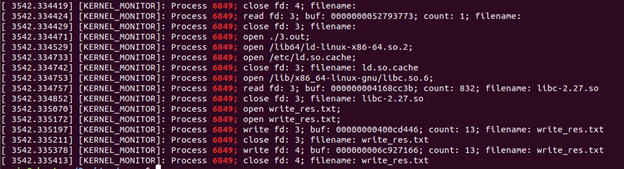
\includegraphics[width = 0.7 \textwidth]{lab_03_3out.png}
        \caption{Пример работы загружаемого модуля ядра.}
        \label{3out}
    \end{figure}

\section{Вывод}
    В данном разделе был обоснован выбор языка программирования, 
    рассмотрены листинги реализованных функций. 
    Приведены результаты работы ПО.

\pagebreak